\documentclass{standalone}
\usepackage{tikz}
\usetikzlibrary{tqft,calc}

\begin{document}

{\scriptsize
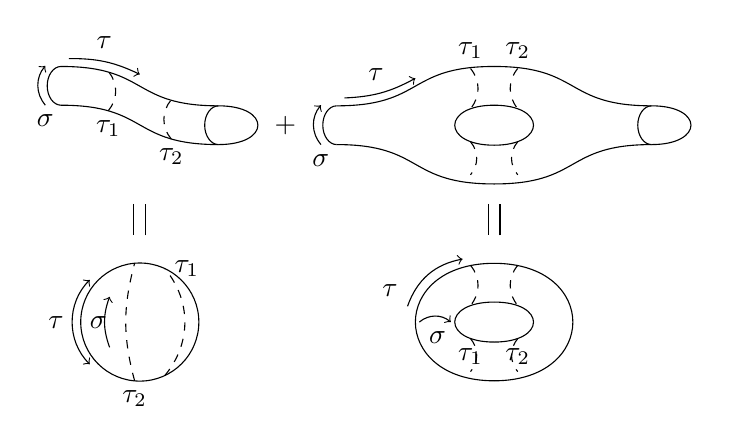
\begin{tikzpicture}[every tqft/.append style={transform shape, rotate=90, tqft/circle x radius=7pt, tqft/boundary separation=1cm, tqft/view from=incoming}]
  % cobordism at upper left
  \pic[
    tqft/cylinder to prior,
    name=a,
    every incoming lower boundary component/.style={draw},
    every outgoing lower boundary component/.style={draw},
    cobordism  edge/.style={draw},
  ];
  \pic[
    tqft/cup,
    cobordism  edge/.style={draw},
    at=(a-outgoing boundary),
  ];
  % annotation of cobordism at upper left
  \coordinate (temp1) at ($(a-incoming  boundary.west)!0.3!(a-outgoing  boundary.west) +(0,0.08)$);
  \coordinate (temp2) at ($(a-incoming  boundary.west)!0.7!(a-outgoing  boundary.west) +(0,-0.08)$);
  \draw[dashed]
  (temp1) node[below] {$\tau_1$} to[bend right=40] ++(0,0.5)
  (temp2) node[below] {$\tau_2$} to[bend left=40] ++(0,0.5);
  \draw[->] ($(a-incoming boundary.west) - (0.2,0)$) node[below] {$\sigma$} to[bend left=40] ++(0,0.5);
  \draw (a-outgoing boundary) ++(0.85,0) node {$+$};
  \draw[->] ($(a-incoming  boundary.east)+(0.1,0.1)$) to[bend left=13] +(0.9,-0.2);
  \node[above] at ($(a-incoming  boundary.east)+(0.55,0.1)$) {$\tau$};
  %
  % cobordism at upper right consisting of two 'pants' and a cup
  \pic[
    tqft/pair of pants,
    name=b,
    every incoming lower boundary component/.style={draw},
    cobordism  edge/.style={draw},
    at={($(a-outgoing boundary)+(1.5,0)$)},
  ];
  %
  \pic[
    tqft/reverse pair of pants,
    name=c,
    every outgoing lower boundary component/.style={draw},
    cobordism  edge/.style={draw},
    at=(b-outgoing boundary 1),
  ];
  \pic[
    tqft/cup,
    cobordism  edge/.style={draw},
    at=(c-outgoing boundary),
  ];
  %  annotation of cobordism at upper right
  \draw[->] ($(b-incoming boundary.west) - (0.2,0)$) node[below] {$\sigma$}  to[bend left=40] ++(0,0.5);
  \coordinate (temp1) at ($(b-between outgoing 1 and 2)!0.2!(c-between incoming 1 and 2) +(0,0.72)$);
  \coordinate (temp2) at ($(b-between outgoing 1 and 2)!0.8!(c-between incoming 1 and 2) +(0,0.72)$);
  \draw[dashed]
  (temp1) node[above] {$\tau_1$} to[bend left=40] +(0,-0.51) ++(0,-0.93) to[bend left=40] ++(0,-0.42)
  (temp2) node[above] {$\tau_2$} to[bend right=40] +(0,-0.51) ++(0,-0.93) to[bend right=40] ++(0,-0.42);
  \draw[->] ($(b-incoming  boundary.east)+(0.1,0.1)$) to[bend right=13] +(0.9,0.25);
  \node[above] at ($(b-incoming  boundary.east)+(0.5,0.2)$) {$\tau$};
  %
  %drawing ring
  \pic[
    tqft ,
    name=d,
    incoming boundary components=0,
    outgoing boundary components=2,
    cobordism  edge/.style={draw},
    anchor=between outgoing 1 and 2,
    at={($(b-between outgoing 1 and 2)!0!(c-between incoming 1 and 2) - (0,2.5)$)},
  ];

  \pic[
    tqft ,
    name=e,
    incoming boundary components=2,
    outgoing boundary components=0,
    cobordism  edge/.style={draw},
    at = {(d-outgoing boundary 1)},
  ];
  \coordinate (temp1) at ($(d-between outgoing 1 and 2)!0.2!(e-between incoming 1 and 2) +(0,0.72)$);
  \coordinate (temp2) at ($(d-between outgoing 1 and 2)!0.8!(e-between incoming 1 and 2) +(0,0.72)$);
  \draw[dashed]
  (temp1) to[bend left=40] +(0,-0.51) ++(0,-0.93) node[below] {$\tau_1$} to[bend left=40] ++(0,-0.42)
  (temp2) to[bend right=40] +(0,-0.51) ++(0,-0.93) node[below] {$\tau_2$} to[bend right=40] ++(0,-0.42);
  %
  \coordinate (temp1) at ($(d-between outgoing 1 and 2)!0.5!(e-between incoming 1 and 2)$);
  \coordinate (temp2) at (a-between first incoming and first outgoing);
  \draw[->] ($(e-incoming boundary 2)+(-1.1,-0.3)$) node[above left] {$\tau$} to[bend left=30] +(0.7,0.6);
  \draw [->] ($(d-between outgoing 1 and 2) + (-0.45,0)$) node [below right] {$\sigma$} to[bend left=40] +(0.4,0);
  \draw (temp1) ++(-0.075,1.5) -- ++(0,-0.4) ++(0.15,0) -- +(0,0.4);
  %
  % drawing and annotating ball
  \node[draw, shape=circle, minimum width=1.5cm]
  at (temp1-|temp2)  (circ){};
  \draw[dashed] (circ) +(265:0.75) node[below] {$\tau_2$} to[bend left=15] +(95:0.75);
  \draw[dashed] (circ) +(295:0.75) to[bend right=40] +(65:0.75) node[right] {$\tau_1$};
  \draw[->] (circ) +(220:0.5) to[bend left=20] +(140:0.5);
  \node[right] at(circ.west) {$\sigma$};
  \draw (circ) ++(-0.075,1.5) -- ++(0,-0.4) ++(0.15,0) -- +(0,0.4);
  \draw[<->] (circ.south west) +(-0.1,0) to[bend left=45] ($(circ.north west)+(-0.1,0)$);
  \node[left=0.25em] at(circ.west) {$\tau$};
\end{tikzpicture}
}

\end{document}